\section{Confidence intervals and the second corpus}\label{app:ci}
All numbers here come from \texttt{exp\_z2\_ci}, an implementation of the family sweep written from the description in Sections~\ref{sec:method} and~\ref{sec:setup} independently of the individual experiment scripts, run under one protocol for all eight models: 32{,}768 evaluation states per model and corpus, the same three dictionaries, OMP with $k=64$ read at 32 and 64, one-shot attribution, and a bootstrap over the 64 evaluation sequences with 1{,}000 resamples. Brackets are 95\% percentile intervals. GPT-2 keeps the conventions of Section~\ref{sec:setup} (a disjoint centering slice for reconstruction, the evaluation mean for attribution); the other families center on eight disjoint chunks throughout. Table~\ref{app:ci-old} sets its point estimates beside those of the individual experiment scripts.
\begin{table}[H]\centering\scriptsize
\caption{Reconstruction of the typical states on WikiText-2 with 95\% bootstrap intervals over sequences. Off top-5 removes the five highest-variance coordinates from numerator and denominator.}\label{app:ci-recon-wikitext}
\begin{adjustbox}{max width=\linewidth}
\begin{tabular}{lrrrrrrrr}\toprule
Model & FVU@32 weight & FVU@64 weight & FVU@32 rotated & FVU@64 rotated & FVU@32 random & off top-5, weight & off top-5, rotated & top-5 share \\ \midrule
GPT-2 small & 0.338 [0.337, 0.340] & 0.179 [0.179, 0.180] & 0.529 [0.529, 0.530] & 0.288 & 0.500 [0.500, 0.500] & 0.38 & 0.56 & 82.1\% \\
SmolLM2-135M & 0.269 [0.268, 0.270] & 0.113 [0.113, 0.114] & 0.421 [0.421, 0.422] & 0.179 & 0.383 [0.383, 0.383] & 0.34 & 0.49 & 98.2\% \\
Qwen2.5-0.5B & 0.408 [0.407, 0.408] & 0.219 [0.219, 0.219] & 0.527 [0.527, 0.527] & 0.282 & 0.512 [0.512, 0.512] & 0.44 & 0.55 & 95.4\% \\
Pythia-410m & 0.503 [0.502, 0.504] & 0.303 [0.302, 0.303] & 0.592 [0.592, 0.592] & 0.359 & 0.586 [0.586, 0.587] & 0.54 & 0.62 & 91.3\% \\
OLMo-1B & 0.563 [0.561, 0.564] & 0.435 [0.433, 0.436] & 0.773 [0.773, 0.773] & 0.611 & 0.771 [0.771, 0.771] & 0.60 & 0.79 & 96.7\% \\
Qwen2.5-7B & 0.555 [0.551, 0.558] & 0.459 [0.456, 0.462] & 0.847 [0.847, 0.847] & 0.729 & 0.846 [0.846, 0.846] & 0.68 & 0.88 & 95.8\% \\
Llama-7B & 0.631 [0.628, 0.633] & 0.533 [0.531, 0.535] & 0.872 [0.872, 0.872] & 0.772 & 0.872 [0.872, 0.872] & 0.66 & 0.88 & 86.9\% \\
Pythia-6.9B & 0.711 [0.709, 0.713] & 0.610 [0.609, 0.612] & 0.868 [0.868, 0.868] & 0.764 & 0.867 [0.867, 0.867] & 0.74 & 0.87 & 55.9\% \\
\bottomrule\end{tabular}\end{adjustbox}
\end{table}
\begin{table}[H]\centering\scriptsize
\caption{The sink states on WikiText-2: how many of the 32{,}768 states exceed ten times the median norm, the variance they carry, and their reconstruction. The all-state columns are what an FVU over all states reports.}\label{app:ci-sink-wikitext}
\begin{adjustbox}{max width=\linewidth}
\begin{tabular}{lrrrrrrrr}\toprule
Model & sink states & smallest sink norm over median & share of variance & sink FVU@32 weight & rotated & random & all-state FVU@32 weight & rotated \\ \midrule
GPT-2 small & 64 & 44$\times$ & 79.7\% & 0.0003 [0.0003, 0.0003] & 0.532 & 0.508 & 0.069 & 0.531 \\
SmolLM2-135M & 64 & 155$\times$ & 98.1\% & 0.0005 [0.0005, 0.0005] & 0.421 & 0.390 & 0.006 & 0.421 \\
Qwen2.5-0.5B & 65 & 85$\times$ & 96.2\% & 0.0013 [0.0013, 0.0013] & 0.517 & 0.514 & 0.017 & 0.518 \\
Pythia-410m & 127 & 47$\times$ & 90.8\% & 0.0037 [0.0037, 0.0037] & 0.591 & 0.582 & 0.050 & 0.591 \\
OLMo-1B & 68 & 43$\times$ & 96.8\% & 0.0006 [0.0006, 0.0006] & 0.779 & 0.773 & 0.019 & 0.779 \\
Qwen2.5-7B & 65 & 203$\times$ & 99.0\% & 0.0039 [0.0038, 0.0040] & 0.840 & 0.843 & 0.010 & 0.840 \\
Llama-7B & 131 & 27$\times$ & 86.0\% & 0.0002 [0.0002, 0.0002] & 0.870 & 0.870 & 0.089 & 0.870 \\
Pythia-6.9B & 66 & 21$\times$ & 58.7\% & 0.0270 [0.0269, 0.0272] & 0.873 & 0.866 & 0.310 & 0.871 \\
\bottomrule\end{tabular}\end{adjustbox}
\end{table}
\begin{table}[H]\centering\scriptsize
\caption{Attribution on WikiText-2 with 95\% bootstrap intervals over sequences. The all-state correlations are carried by the few identified writes at the sink states, whose magnitudes dominate the statistic; the typical-state columns exclude them, and Table~\ref{app:ci-calib-wikitext} is the accuracy statement.}\label{app:ci-attrib-wikitext}
\begin{adjustbox}{max width=\linewidth}
\begin{tabular}{lrrrrrrrr}\toprule
Model & gated & top-1 recall, OMP & top-1 recall, one-shot & $r$ identified, all states & typical states & $r$ unconditional, all & typical & identified writes \\ \midrule
GPT-2 small & no & 0.647 [0.637, 0.657] & 0.766 [0.754, 0.776] & 0.998 [0.998, 0.998] & 0.582 & 0.648 [0.648, 0.648] & 0.505 & 48,220 \\
SmolLM2-135M & yes & 0.670 [0.661, 0.680] & 0.682 [0.676, 0.688] & 1.000 [1.000, 1.000] & 0.835 & 0.928 [0.927, 0.928] & 0.494 & 48,543 \\
Qwen2.5-0.5B & yes & 0.459 [0.451, 0.467] & 0.614 [0.604, 0.623] & 0.994 [0.993, 0.994] & 0.819 & 0.551 [0.543, 0.559] & 0.534 & 34,285 \\
Pythia-410m & no & 0.481 [0.472, 0.490] & 0.593 [0.584, 0.601] & 0.980 [0.979, 0.981] & 0.322 & 0.452 [0.446, 0.455] & 0.275 & 35,864 \\
OLMo-1B & yes & 0.693 [0.687, 0.699] & 0.779 [0.775, 0.784] & 0.997 [0.997, 0.998] & 0.907 & 0.971 [0.969, 0.972] & 0.762 & 59,579 \\
Qwen2.5-7B & yes & 0.673 [0.663, 0.685] & 0.004 [0.004, 0.005] & 0.554 [0.506, 0.595] & 0.887 & 0.308 [0.271, 0.343] & 0.742 & 54,625 \\
Llama-7B & yes & 0.981 [0.979, 0.983] & 0.895 [0.881, 0.906] & 0.999 [0.999, 0.999] & 0.982 & 0.998 [0.998, 0.998] & 0.970 & 93,027 \\
Pythia-6.9B & no & 0.787 [0.779, 0.795] & 0.646 [0.639, 0.653] & 0.539 [0.528, 0.551] & 0.645 & 0.424 [0.409, 0.439] & 0.482 & 67,509 \\
\bottomrule\end{tabular}\end{adjustbox}
\end{table}
\begin{table}[H]\centering\scriptsize
\caption{Calibration of the recovered coefficients of identified dominant writes on WikiText-2, typical states. Ratio is recovered over true; a ratio above one is over-estimation.}\label{app:ci-calib-wikitext}
\begin{adjustbox}{max width=\linewidth}
\begin{tabular}{lrrrrrrrrrrr}\toprule
Model & identified writes & negative & sign recovered & median relative error & within 25\% & ratio, decile 1 & 5 & 10 & rel. error, decile 1 & 5 & 10 \\ \midrule
GPT-2 small & 48,156 & 0\% & 99.8\% & 0.44 [0.44, 0.45] & 29.4\% & 1.66 & 1.42 & 1.45 & 0.66 & 0.42 & 0.45 \\
SmolLM2-135M & 48,479 & 50\% & 100.0\% & 0.54 [0.53, 0.54] & 26.0\% & 1.97 & 1.55 & 0.73 & 0.97 & 0.55 & 0.32 \\
Qwen2.5-0.5B & 34,220 & 47\% & 100.0\% & 0.46 [0.45, 0.46] & 26.5\% & 1.58 & 1.34 & 0.43 & 0.58 & 0.45 & 0.57 \\
Pythia-410m & 35,801 & 0\% & 99.9\% & 0.41 [0.40, 0.42] & 34.2\% & 1.75 & 1.43 & 1.04 & 0.75 & 0.43 & 0.27 \\
OLMo-1B & 59,503 & 46\% & 99.7\% & 0.34 [0.34, 0.34] & 35.0\% & 1.06 & 0.76 & 0.51 & 0.25 & 0.32 & 0.49 \\
Qwen2.5-7B & 54,601 & 51\% & 100.0\% & 0.50 [0.50, 0.51] & 17.6\% & 0.97 & 0.52 & 0.29 & 0.25 & 0.48 & 0.71 \\
Llama-7B & 92,755 & 49\% & 100.0\% & 0.25 [0.25, 0.25] & 49.8\% & 1.39 & 1.24 & 1.17 & 0.39 & 0.26 & 0.17 \\
Pythia-6.9B & 67,475 & 0\% & 100.0\% & 1.03 [1.02, 1.04] & 4.4\% & 2.19 & 2.03 & 1.86 & 1.19 & 1.03 & 0.86 \\
\bottomrule\end{tabular}\end{adjustbox}
\end{table}
\begin{table}[H]\centering\scriptsize
\caption{Within-decile correlation of recovered and true coefficients on WikiText-2 (point estimates; intervals in Figure~\ref{app:ci-decilefig-wikitext}). In the gated models about half of the writes are negative, so this signed correlation within a magnitude decile mostly records sign recovery, and Table~\ref{app:ci-calib-wikitext} is the accuracy statement.}\label{app:ci-deciles-wikitext}
\begin{adjustbox}{max width=\linewidth}
\begin{tabular}{lrrrrrrrrrr}\toprule
Model & 1 & 2 & 3 & 4 & 5 & 6 & 7 & 8 & 9 & 10 \\ \midrule
GPT-2 small & 0.05 & 0.04 & 0.03 & 0.00 & 0.06 & 0.02 & 0.02 & 0.13 & 0.24 & 1.00 \\
SmolLM2-135M & 0.94 & 0.92 & 0.94 & 0.95 & 0.94 & 0.93 & 0.94 & 0.94 & 0.93 & 1.00 \\
Qwen2.5-0.5B & 0.94 & 0.93 & 0.91 & 0.91 & 0.91 & 0.92 & 0.90 & 0.88 & 0.94 & 1.00 \\
Pythia-410m & 0.21 & 0.03 & 0.08 & 0.02 & -0.05 & -0.02 & 0.03 & 0.07 & -0.07 & 1.00 \\
OLMo-1B & 0.93 & 0.95 & 0.94 & 0.94 & 0.93 & 0.93 & 0.92 & 0.91 & 0.91 & 1.00 \\
Qwen2.5-7B & 0.94 & 0.95 & 0.94 & 0.94 & 0.94 & 0.94 & 0.94 & 0.94 & 0.94 & 0.70 \\
Llama-7B & 0.97 & 0.98 & 0.98 & 0.98 & 0.98 & 0.98 & 0.98 & 0.98 & 0.99 & 1.00 \\
Pythia-6.9B & 0.22 & 0.02 & 0.04 & 0.04 & 0.05 & 0.07 & 0.04 & 0.08 & 0.12 & 0.66 \\
\bottomrule\end{tabular}\end{adjustbox}
\end{table}
\begin{figure}[H]\centering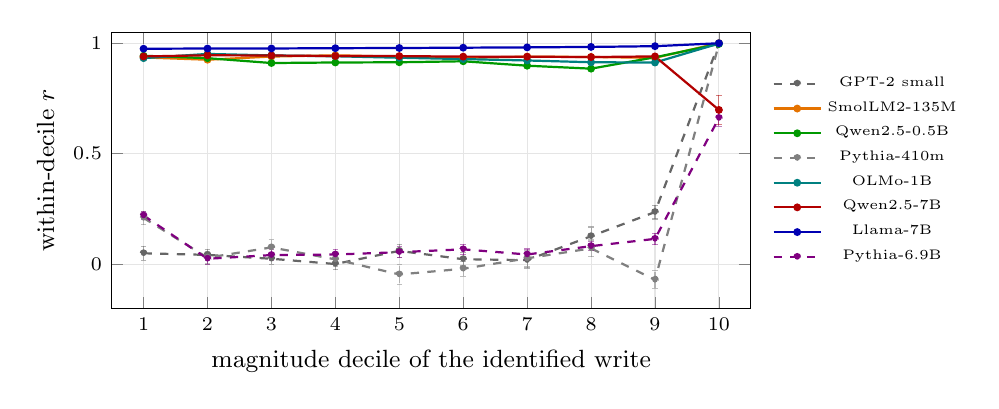
\begin{tikzpicture}\begin{axis}[width=0.8\linewidth, height=0.42\linewidth, xlabel={magnitude decile of the identified write}, ylabel={within-decile $r$}, xmin=0.5, xmax=10.5, ymin=-0.2, ymax=1.05, xtick={1,...,10}, grid=major, grid style={black!10}, legend style={font=\tiny, at={(1.02,0.5)}, anchor=west, draw=none}, tick label style={font=\scriptsize}, label style={font=\small}, error bars/y dir=both, error bars/y explicit]
\addplot[thick, dashed, color=black!60, mark=*, mark size=1pt, error bars/error bar style={opacity=0.5}] coordinates {(1,0.0499) +- (0,0.0322) (2,0.0425) +- (0,0.0256) (3,0.0251) +- (0,0.0254) (4,0.0013) +- (0,0.0260) (5,0.0607) +- (0,0.0294) (6,0.0230) +- (0,0.0301) (7,0.0189) +- (0,0.0354) (8,0.1270) +- (0,0.0416) (9,0.2362) +- (0,0.0312) (10,0.9998) +- (0,0.0000)};\addlegendentry{GPT-2 small}
\addplot[thick, color=orange!90!black, mark=*, mark size=1pt, error bars/error bar style={opacity=0.5}] coordinates {(1,0.9353) +- (0,0.0027) (2,0.9250) +- (0,0.0028) (3,0.9393) +- (0,0.0015) (4,0.9451) +- (0,0.0024) (5,0.9387) +- (0,0.0061) (6,0.9337) +- (0,0.0049) (7,0.9390) +- (0,0.0030) (8,0.9374) +- (0,0.0023) (9,0.9334) +- (0,0.0030) (10,0.9998) +- (0,0.0000)};\addlegendentry{SmolLM2-135M}
\addplot[thick, color=green!60!black, mark=*, mark size=1pt, error bars/error bar style={opacity=0.5}] coordinates {(1,0.9430) +- (0,0.0037) (2,0.9320) +- (0,0.0038) (3,0.9101) +- (0,0.0027) (4,0.9125) +- (0,0.0033) (5,0.9135) +- (0,0.0029) (6,0.9180) +- (0,0.0033) (7,0.8980) +- (0,0.0033) (8,0.8846) +- (0,0.0040) (9,0.9360) +- (0,0.0046) (10,0.9962) +- (0,0.0009)};\addlegendentry{Qwen2.5-0.5B}
\addplot[thick, dashed, color=gray, mark=*, mark size=1pt, error bars/error bar style={opacity=0.5}] coordinates {(1,0.2098) +- (0,0.0308) (2,0.0299) +- (0,0.0286) (3,0.0764) +- (0,0.0343) (4,0.0224) +- (0,0.0321) (5,-0.0458) +- (0,0.0435) (6,-0.0202) +- (0,0.0343) (7,0.0271) +- (0,0.0364) (8,0.0720) +- (0,0.0381) (9,-0.0702) +- (0,0.0402) (10,0.9959) +- (0,0.0004)};\addlegendentry{Pythia-410m}
\addplot[thick, color=teal, mark=*, mark size=1pt, error bars/error bar style={opacity=0.5}] coordinates {(1,0.9322) +- (0,0.0054) (2,0.9512) +- (0,0.0014) (3,0.9445) +- (0,0.0019) (4,0.9406) +- (0,0.0017) (5,0.9340) +- (0,0.0019) (6,0.9279) +- (0,0.0020) (7,0.9216) +- (0,0.0025) (8,0.9136) +- (0,0.0028) (9,0.9123) +- (0,0.0026) (10,0.9982) +- (0,0.0007)};\addlegendentry{OLMo-1B}
\addplot[thick, color=red!70!black, mark=*, mark size=1pt, error bars/error bar style={opacity=0.5}] coordinates {(1,0.9398) +- (0,0.0023) (2,0.9451) +- (0,0.0021) (3,0.9441) +- (0,0.0021) (4,0.9415) +- (0,0.0019) (5,0.9414) +- (0,0.0032) (6,0.9390) +- (0,0.0042) (7,0.9387) +- (0,0.0046) (8,0.9370) +- (0,0.0064) (9,0.9400) +- (0,0.0062) (10,0.6980) +- (0,0.0659)};\addlegendentry{Qwen2.5-7B}
\addplot[thick, color=blue!70!black, mark=*, mark size=1pt, error bars/error bar style={opacity=0.5}] coordinates {(1,0.9747) +- (0,0.0009) (2,0.9756) +- (0,0.0009) (3,0.9759) +- (0,0.0008) (4,0.9771) +- (0,0.0012) (5,0.9780) +- (0,0.0008) (6,0.9794) +- (0,0.0006) (7,0.9808) +- (0,0.0009) (8,0.9829) +- (0,0.0007) (9,0.9862) +- (0,0.0007) (10,0.9995) +- (0,0.0000)};\addlegendentry{Llama-7B}
\addplot[thick, dashed, color=violet, mark=*, mark size=1pt, error bars/error bar style={opacity=0.5}] coordinates {(1,0.2207) +- (0,0.0199) (2,0.0250) +- (0,0.0245) (3,0.0418) +- (0,0.0241) (4,0.0442) +- (0,0.0237) (5,0.0549) +- (0,0.0243) (6,0.0677) +- (0,0.0238) (7,0.0444) +- (0,0.0247) (8,0.0821) +- (0,0.0198) (9,0.1150) +- (0,0.0256) (10,0.6616) +- (0,0.0405)};\addlegendentry{Pythia-6.9B}
\end{axis}\end{tikzpicture}\caption{Within-decile correlation per model on WikiText-2, with 95\% bootstrap intervals as error bars. Solid lines are gated-MLP models, dashed non-gated.}\label{app:ci-decilefig-wikitext}\end{figure}
\begin{table}[H]\centering\scriptsize
\caption{Reconstruction of the typical states on the Pile sample with 95\% bootstrap intervals over sequences. Off top-5 removes the five highest-variance coordinates from numerator and denominator.}\label{app:ci-recon-pile}
\begin{adjustbox}{max width=\linewidth}
\begin{tabular}{lrrrrrrrr}\toprule
Model & FVU@32 weight & FVU@64 weight & FVU@32 rotated & FVU@64 rotated & FVU@32 random & off top-5, weight & off top-5, rotated & top-5 share \\ \midrule
GPT-2 small & 0.358 [0.354, 0.362] & 0.190 [0.188, 0.192] & 0.530 [0.529, 0.530] & 0.288 & 0.500 [0.500, 0.500] & 0.40 & 0.56 & 80.6\% \\
SmolLM2-135M & 0.277 [0.276, 0.279] & 0.117 [0.116, 0.117] & 0.421 [0.421, 0.421] & 0.179 & 0.383 [0.383, 0.383] & 0.35 & 0.49 & 98.2\% \\
Qwen2.5-0.5B & 0.413 [0.411, 0.415] & 0.222 [0.221, 0.223] & 0.528 [0.527, 0.528] & 0.282 & 0.512 [0.512, 0.512] & 0.44 & 0.55 & 95.2\% \\
Pythia-410m & 0.509 [0.507, 0.511] & 0.306 [0.305, 0.307] & 0.592 [0.592, 0.593] & 0.359 & 0.586 [0.586, 0.587] & 0.55 & 0.62 & 91.5\% \\
OLMo-1B & 0.503 [0.502, 0.505] & 0.388 [0.387, 0.389] & 0.773 [0.773, 0.773] & 0.610 & 0.771 [0.771, 0.771] & 0.60 & 0.81 & 98.2\% \\
Qwen2.5-7B & 0.533 [0.530, 0.536] & 0.438 [0.436, 0.440] & 0.847 [0.847, 0.847] & 0.729 & 0.846 [0.846, 0.846] & 0.66 & 0.88 & 95.7\% \\
Llama-7B & 0.627 [0.625, 0.629] & 0.529 [0.527, 0.531] & 0.872 [0.872, 0.872] & 0.772 & 0.872 [0.872, 0.872] & 0.65 & 0.88 & 85.1\% \\
Pythia-6.9B & 0.682 [0.677, 0.688] & 0.584 [0.579, 0.588] & 0.868 [0.868, 0.868] & 0.764 & 0.867 [0.867, 0.867] & 0.72 & 0.88 & 65.5\% \\
\bottomrule\end{tabular}\end{adjustbox}
\end{table}
\begin{table}[H]\centering\scriptsize
\caption{The sink states on the Pile sample: how many of the 32{,}768 states exceed ten times the median norm, the variance they carry, and their reconstruction. The all-state columns are what an FVU over all states reports.}\label{app:ci-sink-pile}
\begin{adjustbox}{max width=\linewidth}
\begin{tabular}{lrrrrrrrr}\toprule
Model & sink states & smallest sink norm over median & share of variance & sink FVU@32 weight & rotated & random & all-state FVU@32 weight & rotated \\ \midrule
GPT-2 small & 64 & 41$\times$ & 77.9\% & 0.0003 [0.0003, 0.0003] & 0.533 & 0.507 & 0.079 & 0.532 \\
SmolLM2-135M & 66 & 158$\times$ & 98.1\% & 0.0005 [0.0005, 0.0005] & 0.421 & 0.390 & 0.006 & 0.421 \\
Qwen2.5-0.5B & 64 & 102$\times$ & 96.0\% & 0.0013 [0.0013, 0.0014] & 0.517 & 0.514 & 0.018 & 0.517 \\
Pythia-410m & 129 & 41$\times$ & 91.2\% & 0.0037 [0.0037, 0.0038] & 0.591 & 0.582 & 0.048 & 0.591 \\
OLMo-1B & 173 & 33$\times$ & 98.4\% & 0.0005 [0.0004, 0.0005] & 0.778 & 0.774 & 0.009 & 0.778 \\
Qwen2.5-7B & 64 & 124$\times$ & 98.9\% & 0.0039 [0.0038, 0.0040] & 0.840 & 0.843 & 0.010 & 0.840 \\
Llama-7B & 132 & 10$\times$ & 84.3\% & 0.0002 [0.0002, 0.0002] & 0.870 & 0.870 & 0.098 & 0.870 \\
Pythia-6.9B & 129 & 10$\times$ & 69.2\% & 0.0269 [0.0268, 0.0270] & 0.873 & 0.866 & 0.229 & 0.872 \\
\bottomrule\end{tabular}\end{adjustbox}
\end{table}
\begin{table}[H]\centering\scriptsize
\caption{Attribution on the Pile sample with 95\% bootstrap intervals over sequences. The all-state correlations are carried by the few identified writes at the sink states, whose magnitudes dominate the statistic; the typical-state columns exclude them, and Table~\ref{app:ci-calib-pile} is the accuracy statement.}\label{app:ci-attrib-pile}
\begin{adjustbox}{max width=\linewidth}
\begin{tabular}{lrrrrrrrr}\toprule
Model & gated & top-1 recall, OMP & top-1 recall, one-shot & $r$ identified, all states & typical states & $r$ unconditional, all & typical & identified writes \\ \midrule
GPT-2 small & no & 0.568 [0.546, 0.588] & 0.665 [0.632, 0.696] & 0.998 [0.998, 0.998] & 0.557 & 0.647 [0.647, 0.647] & 0.449 & 43,180 \\
SmolLM2-135M & yes & 0.663 [0.651, 0.675] & 0.710 [0.696, 0.723] & 1.000 [1.000, 1.000] & 0.864 & 0.927 [0.926, 0.928] & 0.472 & 48,024 \\
Qwen2.5-0.5B & yes & 0.483 [0.470, 0.495] & 0.623 [0.606, 0.641] & 0.995 [0.995, 0.995] & 0.830 & 0.542 [0.536, 0.547] & 0.546 & 35,927 \\
Pythia-410m & no & 0.460 [0.448, 0.472] & 0.608 [0.586, 0.629] & 0.978 [0.976, 0.979] & 0.300 & 0.447 [0.434, 0.456] & 0.288 & 33,977 \\
OLMo-1B & yes & 0.735 [0.727, 0.743] & 0.756 [0.749, 0.764] & 0.996 [0.995, 0.996] & 0.915 & 0.977 [0.977, 0.978] & 0.787 & 62,804 \\
Qwen2.5-7B & yes & 0.689 [0.677, 0.701] & 0.004 [0.003, 0.004] & 0.526 [0.482, 0.570] & 0.882 & 0.286 [0.253, 0.321] & 0.755 & 56,793 \\
Llama-7B & yes & 0.980 [0.978, 0.982] & 0.905 [0.898, 0.912] & 0.999 [0.999, 0.999] & 0.984 & 0.998 [0.998, 0.998] & 0.974 & 93,181 \\
Pythia-6.9B & no & 0.759 [0.740, 0.775] & 0.526 [0.507, 0.546] & 0.548 [0.527, 0.579] & 0.674 & 0.295 [0.280, 0.311] & 0.399 & 65,746 \\
\bottomrule\end{tabular}\end{adjustbox}
\end{table}
\begin{table}[H]\centering\scriptsize
\caption{Calibration of the recovered coefficients of identified dominant writes on the Pile sample, typical states. Ratio is recovered over true; a ratio above one is over-estimation.}\label{app:ci-calib-pile}
\begin{adjustbox}{max width=\linewidth}
\begin{tabular}{lrrrrrrrrrrr}\toprule
Model & identified writes & negative & sign recovered & median relative error & within 25\% & ratio, decile 1 & 5 & 10 & rel. error, decile 1 & 5 & 10 \\ \midrule
GPT-2 small & 43,116 & 0\% & 99.7\% & 0.51 [0.50, 0.52] & 24.1\% & 1.68 & 1.48 & 1.50 & 0.69 & 0.49 & 0.51 \\
SmolLM2-135M & 47,958 & 51\% & 100.0\% & 0.58 [0.57, 0.59] & 24.1\% & 1.99 & 1.86 & 0.86 & 1.00 & 0.87 & 0.31 \\
Qwen2.5-0.5B & 35,863 & 52\% & 100.0\% & 0.44 [0.44, 0.44] & 28.2\% & 1.75 & 1.30 & 0.48 & 0.75 & 0.43 & 0.52 \\
Pythia-410m & 33,915 & 0\% & 99.9\% & 0.39 [0.38, 0.41] & 34.4\% & 1.77 & 1.40 & 0.92 & 0.77 & 0.41 & 0.28 \\
OLMo-1B & 62,540 & 47\% & 100.0\% & 0.32 [0.32, 0.32] & 37.8\% & 1.12 & 0.80 & 0.54 & 0.24 & 0.29 & 0.46 \\
Qwen2.5-7B & 56,777 & 53\% & 100.0\% & 0.46 [0.45, 0.47] & 21.3\% & 1.10 & 0.58 & 0.33 & 0.27 & 0.43 & 0.67 \\
Llama-7B & 92,889 & 50\% & 100.0\% & 0.29 [0.28, 0.29] & 42.9\% & 1.47 & 1.29 & 1.19 & 0.47 & 0.30 & 0.20 \\
Pythia-6.9B & 65,725 & 0\% & 99.9\% & 1.08 [1.07, 1.09] & 3.8\% & 2.26 & 2.09 & 1.85 & 1.26 & 1.09 & 0.85 \\
\bottomrule\end{tabular}\end{adjustbox}
\end{table}
\begin{table}[H]\centering\scriptsize
\caption{Within-decile correlation of recovered and true coefficients on the Pile sample (point estimates; intervals in Figure~\ref{app:ci-decilefig-pile}). In the gated models about half of the writes are negative, so this signed correlation within a magnitude decile mostly records sign recovery, and Table~\ref{app:ci-calib-pile} is the accuracy statement.}\label{app:ci-deciles-pile}
\begin{adjustbox}{max width=\linewidth}
\begin{tabular}{lrrrrrrrrrr}\toprule
Model & 1 & 2 & 3 & 4 & 5 & 6 & 7 & 8 & 9 & 10 \\ \midrule
GPT-2 small & 0.05 & 0.07 & 0.00 & 0.04 & 0.01 & 0.06 & 0.03 & 0.07 & 0.15 & 1.00 \\
SmolLM2-135M & 0.94 & 0.94 & 0.94 & 0.94 & 0.94 & 0.93 & 0.94 & 0.95 & 0.94 & 1.00 \\
Qwen2.5-0.5B & 0.92 & 0.92 & 0.91 & 0.91 & 0.91 & 0.91 & 0.90 & 0.89 & 0.93 & 1.00 \\
Pythia-410m & 0.18 & -0.00 & 0.05 & 0.02 & 0.01 & 0.00 & 0.00 & 0.04 & 0.20 & 1.00 \\
OLMo-1B & 0.95 & 0.96 & 0.95 & 0.95 & 0.94 & 0.94 & 0.93 & 0.93 & 0.92 & 1.00 \\
Qwen2.5-7B & 0.93 & 0.94 & 0.94 & 0.94 & 0.94 & 0.93 & 0.94 & 0.93 & 0.93 & 0.63 \\
Llama-7B & 0.98 & 0.98 & 0.98 & 0.98 & 0.98 & 0.98 & 0.98 & 0.99 & 0.99 & 1.00 \\
Pythia-6.9B & 0.18 & 0.07 & 0.08 & 0.04 & 0.04 & 0.04 & 0.05 & 0.09 & 0.11 & 0.54 \\
\bottomrule\end{tabular}\end{adjustbox}
\end{table}
\begin{figure}[H]\centering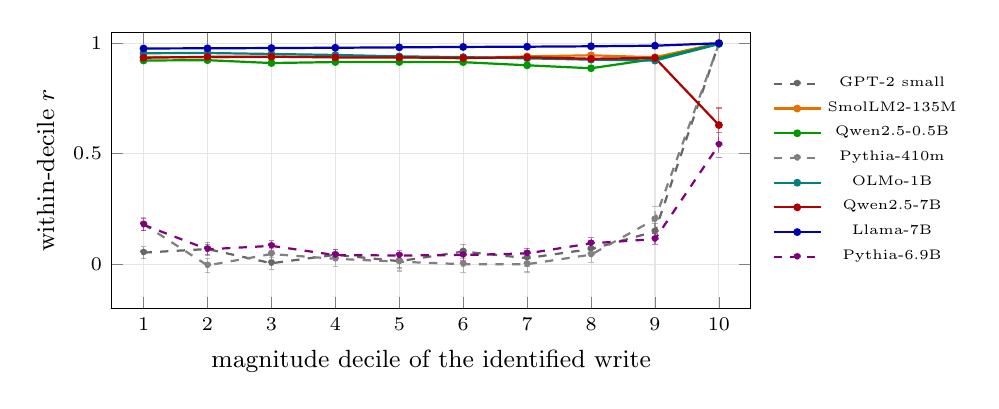
\begin{tikzpicture}\begin{axis}[width=0.8\linewidth, height=0.42\linewidth, xlabel={magnitude decile of the identified write}, ylabel={within-decile $r$}, xmin=0.5, xmax=10.5, ymin=-0.2, ymax=1.05, xtick={1,...,10}, grid=major, grid style={black!10}, legend style={font=\tiny, at={(1.02,0.5)}, anchor=west, draw=none}, tick label style={font=\scriptsize}, label style={font=\small}, error bars/y dir=both, error bars/y explicit]
\addplot[thick, dashed, color=black!60, mark=*, mark size=1pt, error bars/error bar style={opacity=0.5}] coordinates {(1,0.0528) +- (0,0.0276) (2,0.0690) +- (0,0.0305) (3,0.0048) +- (0,0.0267) (4,0.0430) +- (0,0.0248) (5,0.0142) +- (0,0.0311) (6,0.0576) +- (0,0.0325) (7,0.0280) +- (0,0.0357) (8,0.0690) +- (0,0.0301) (9,0.1484) +- (0,0.0368) (10,0.9998) +- (0,0.0000)};\addlegendentry{GPT-2 small}
\addplot[thick, color=orange!90!black, mark=*, mark size=1pt, error bars/error bar style={opacity=0.5}] coordinates {(1,0.9375) +- (0,0.0030) (2,0.9360) +- (0,0.0032) (3,0.9379) +- (0,0.0024) (4,0.9387) +- (0,0.0029) (5,0.9371) +- (0,0.0034) (6,0.9315) +- (0,0.0035) (7,0.9399) +- (0,0.0023) (8,0.9451) +- (0,0.0021) (9,0.9361) +- (0,0.0022) (10,0.9999) +- (0,0.0000)};\addlegendentry{SmolLM2-135M}
\addplot[thick, color=green!60!black, mark=*, mark size=1pt, error bars/error bar style={opacity=0.5}] coordinates {(1,0.9214) +- (0,0.0031) (2,0.9230) +- (0,0.0035) (3,0.9100) +- (0,0.0036) (4,0.9145) +- (0,0.0028) (5,0.9148) +- (0,0.0023) (6,0.9140) +- (0,0.0045) (7,0.8998) +- (0,0.0032) (8,0.8864) +- (0,0.0040) (9,0.9285) +- (0,0.0058) (10,0.9975) +- (0,0.0003)};\addlegendentry{Qwen2.5-0.5B}
\addplot[thick, dashed, color=gray, mark=*, mark size=1pt, error bars/error bar style={opacity=0.5}] coordinates {(1,0.1817) +- (0,0.0300) (2,-0.0050) +- (0,0.0328) (3,0.0464) +- (0,0.0252) (4,0.0249) +- (0,0.0346) (5,0.0118) +- (0,0.0421) (6,0.0004) +- (0,0.0356) (7,0.0005) +- (0,0.0351) (8,0.0437) +- (0,0.0340) (9,0.2037) +- (0,0.0590) (10,0.9963) +- (0,0.0005)};\addlegendentry{Pythia-410m}
\addplot[thick, color=teal, mark=*, mark size=1pt, error bars/error bar style={opacity=0.5}] coordinates {(1,0.9545) +- (0,0.0021) (2,0.9554) +- (0,0.0013) (3,0.9510) +- (0,0.0016) (4,0.9465) +- (0,0.0016) (5,0.9402) +- (0,0.0019) (6,0.9366) +- (0,0.0017) (7,0.9313) +- (0,0.0023) (8,0.9253) +- (0,0.0022) (9,0.9211) +- (0,0.0025) (10,0.9961) +- (0,0.0005)};\addlegendentry{OLMo-1B}
\addplot[thick, color=red!70!black, mark=*, mark size=1pt, error bars/error bar style={opacity=0.5}] coordinates {(1,0.9339) +- (0,0.0031) (2,0.9381) +- (0,0.0028) (3,0.9387) +- (0,0.0043) (4,0.9355) +- (0,0.0046) (5,0.9351) +- (0,0.0048) (6,0.9330) +- (0,0.0056) (7,0.9360) +- (0,0.0045) (8,0.9295) +- (0,0.0060) (9,0.9331) +- (0,0.0073) (10,0.6297) +- (0,0.0771)};\addlegendentry{Qwen2.5-7B}
\addplot[thick, color=blue!70!black, mark=*, mark size=1pt, error bars/error bar style={opacity=0.5}] coordinates {(1,0.9759) +- (0,0.0008) (2,0.9767) +- (0,0.0008) (3,0.9778) +- (0,0.0007) (4,0.9791) +- (0,0.0006) (5,0.9809) +- (0,0.0007) (6,0.9828) +- (0,0.0012) (7,0.9839) +- (0,0.0009) (8,0.9857) +- (0,0.0008) (9,0.9884) +- (0,0.0008) (10,0.9995) +- (0,0.0000)};\addlegendentry{Llama-7B}
\addplot[thick, dashed, color=violet, mark=*, mark size=1pt, error bars/error bar style={opacity=0.5}] coordinates {(1,0.1787) +- (0,0.0266) (2,0.0679) +- (0,0.0234) (3,0.0834) +- (0,0.0232) (4,0.0417) +- (0,0.0246) (5,0.0398) +- (0,0.0210) (6,0.0419) +- (0,0.0251) (7,0.0492) +- (0,0.0235) (8,0.0948) +- (0,0.0248) (9,0.1140) +- (0,0.0234) (10,0.5402) +- (0,0.0556)};\addlegendentry{Pythia-6.9B}
\end{axis}\end{tikzpicture}\caption{Within-decile correlation per model on the Pile sample, with 95\% bootstrap intervals as error bars. Solid lines are gated-MLP models, dashed non-gated.}\label{app:ci-decilefig-pile}\end{figure}
\begin{table}[H]\centering\scriptsize
\caption{The individual experiment scripts (8{,}192 states for the non-GPT-2 models, corpus-restricted embedding atoms) against the single-protocol sweep on WikiText-2 (32{,}768 states, full-vocabulary dictionaries), both over all states. Agreement within the intervals is the replication check; the remaining differences come from the token sample and the dictionary size.}\label{app:ci-old}
\begin{adjustbox}{max width=\linewidth}
\begin{tabular}{lrrrrrrrr}\toprule
Model & FVU@32, scripts & sweep & recall, scripts & sweep & $r$ id., scripts & sweep & $r$ unc., scripts & sweep \\ \midrule
GPT-2 small & 0.069 & 0.069 [0.068, 0.069] & 0.647 & 0.647 [0.637, 0.657] & 0.998 & 0.998 [0.998, 0.998] & 0.648 & 0.648 [0.648, 0.648] \\
SmolLM2-135M & 0.006 & 0.006 [0.006, 0.006] & 0.673 & 0.670 [0.661, 0.680] & 1.000 & 1.000 [1.000, 1.000] & 0.927 & 0.928 [0.927, 0.928] \\
Qwen2.5-0.5B & 0.018 & 0.017 [0.016, 0.017] & 0.458 & 0.459 [0.451, 0.467] & 0.994 & 0.994 [0.993, 0.994] & 0.556 & 0.551 [0.543, 0.559] \\
Pythia-410m & 0.051 & 0.050 [0.049, 0.051] & 0.470 & 0.481 [0.472, 0.490] & 0.978 & 0.980 [0.979, 0.981] & 0.450 & 0.452 [0.446, 0.455] \\
OLMo-1B & 0.018 & 0.019 [0.018, 0.019] & 0.703 & 0.693 [0.687, 0.699] & 0.996 & 0.997 [0.997, 0.998] & 0.971 & 0.971 [0.969, 0.972] \\
Qwen2.5-7B & 0.010 & 0.010 [0.009, 0.010] & 0.684 & 0.673 [0.663, 0.685] & 0.549 & 0.554 [0.506, 0.595] & 0.312 & 0.308 [0.271, 0.343] \\
Llama-7B & 0.088 & 0.089 [0.087, 0.090] & 0.980 & 0.981 [0.979, 0.983] & 0.999 & 0.999 [0.999, 0.999] & 0.998 & 0.998 [0.998, 0.998] \\
Pythia-6.9B & 0.309 & 0.310 [0.303, 0.315] & 0.808 & 0.787 [0.779, 0.795] & 0.522 & 0.539 [0.528, 0.551] & 0.412 & 0.424 [0.409, 0.439] \\
\bottomrule\end{tabular}\end{adjustbox}
\end{table}
